%
%
%/******************************************************************************
% *filename:		tongxinxieyi.tex
% *author:  		synckey
% *version: 		v1.0
% *datetime:		2011-06-24 11:25:45
% *description:		通信协议
% *****************************************************************************/
%
\section{通信协议}
\subsection{请求报文}
\begin{figure}[H]
\centering
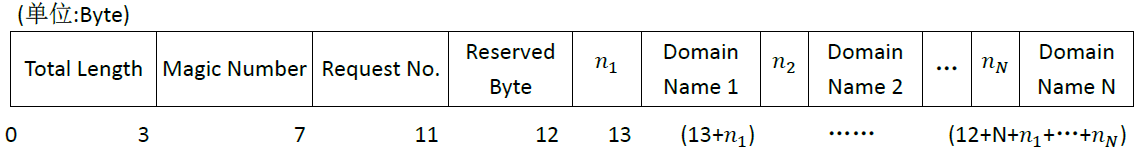
\includegraphics[keepaspectratio, scale=0.4]{pitures/request.png}
\caption{请求报文格式}
\end{figure}
	\begin{asparaitem}
		\item{报文总长度(Total Length)字段:占4字节。用来指定请求报文的总长度。}
		\item{魔数(Magic Number)字段:占4字节。用来区分UDP有效报文和垃圾报文。}
		\item{请求序列号(Request No.)字段:占4字节。用于标示同一台主机向系统请求DNS解析的请求编号。}
		\item{保留字节(Reserved Byte):占1字节。用于返回报文的错误控制、返回顺序等扩展。}
		\item{域名长度($n$)字段:占1字节。用于指定后续字节中域名的长度。}
		\item{域名(Domain Name)字段:不定长字节数。给出要解析的具体域名。}
	\end{asparaitem}

\subsection{返回报文1}
\begin{figure}[H]
\centering
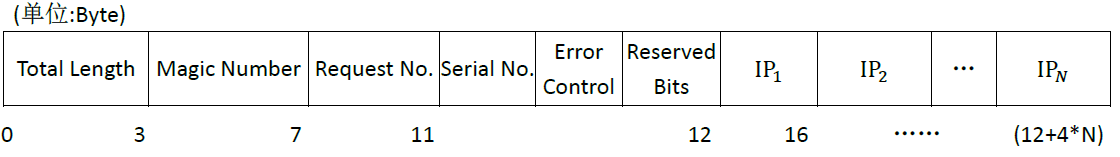
\includegraphics[keepaspectratio,scale=0.4]{pitures/response1.png}
\caption{返回报文1}
\end{figure}
	\begin{asparaitem}
		\item{报文总长度(Total Length)字段:占4字节。用来指定返回报文的总长度。}
		\item{魔数(Magic Number)字段:占4字节。用来区分UDP有效报文和垃圾报文。}
		\item{请求序列号(Request No.)字段:占4字节。用于标示同一台主机向系统请求DNS解析的请求编号。}
		\item{序列号(Serial No.)字段:占1比特。0表示第一次向特定请求返回报文。}
		\item{错误控制(Request No.)字段:占1比特。用于标示后续字节中存在域名解析失败的情况, 0表示
		有错,1表示没有错误。}
		\item{保留字位(Reserved Bits):占6比特。用于返回报文将来可能需要的其他扩展。}
		\item{网际协议地址(IP)字段:占4字节。用于给出请求报文中相应域名的对应IP地址,或者相应的错误代码。}
	\end{asparaitem}

\subsection{返回报文2}
\begin{figure}[H]
\centering
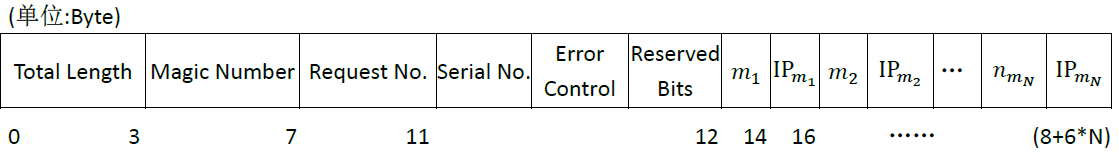
\includegraphics[keepaspectratio,scale=0.4]{pitures/response2.png}
\caption{返回报文2}
\end{figure}
	\begin{asparaitem}
		\item{报文总长度(Total Length)字段:占4字节。用来指定返回报文的总长度。}
		\item{魔数(Magic Number)字段:占4字节。用来区分UDP有效报文和垃圾报文。}
		\item{请求序列号(Request No.)字段:占4字节。用于标示同一台主机向系统请求DNS解析的请求编号。}
		\item{序列号(Serial No.)字段:占1比特。1表示第二次向特定请求返回报文。}
		\item{错误控制(Request No.)字段:占1比特。用于标示后续字节中存在域名解析失败的情况,0表示
		有错,1表示没有错误。}
		\item{保留字位(Reserved Bits):占6比特。用于返回报文将来可能需要的其他扩展。}
		\item{对应位置(m)字段:占4字节。用于给出后续IP地址在请求报文中对应域名的序号。}	
		\item{网际协议地址(IP)字段:占4字节。用于给出请求报文中相应域名的对应IP地址,或者相应的错误代码。}
	\end{asparaitem}

%
%/*********************************  END OF tongxinxieyi.tex  *********************************/
